
For each of the general covariance structures outlined in the previous simulation study description, data were simulated according to multivariate normal distributions with the following covariance matrices: 
\begin{enumerate} 
\item\label{item:cov-type-1} Mutual independence: $\Sigma = \mathrm{I}$, where 
\begin{align*}
\phi\left(t,s\right) &= 0, \quad 0 \le s < t \le 1,\\ 
\sigma^2\left(t\right) &= 1, \quad 0 \le t \le 1.
\end{align*}
\item \label{item:cov-type-2} Linear varying coefficient model with constant innovation variance: $\Sigma^{-1} = T' D^{-1} T$, where 
\begin{align*}
\phi\left(t,s\right) &= t - \frac{1}{2},  \quad 0 \le t \le 1, \\
\sigma^2\left(t\right) &= 0.1^2,  \quad 0 \le t \le 1.
\end{align*}
{\needsparaphrased{TODO: How do we describe the structures for models II-V in terms of continuous $t\in\left[0,1\right]$? }}
\item \label{item:cov-type-3} $k_{1/2}$-banded linear varying coefficient model with constant innovation variance: $\Sigma^{-1} = T' D^{-1} T$, where
\begin{align*}
\phi\left(t,s\right) &= \left\{\begin{array}{ll} t - \frac{1}{2}, & t - s \le 0.5\\ 
0, & t - s > 0.5\end{array}\right.,\\
\sigma^2\left(t\right) &= 0.1^2, \quad 0 \le t \le 1.
\end{align*}
\item \label{item:cov-type-4} $1$-banded linear varying coefficient model with constant innovation variance: $\Sigma^{-1} = T' D^{-1} T$ where 
\begin{align*}
\phi\left(t,s\right) &= \left\{\begin{array}{ll} t - \frac{1}{2}, & t - s \le \frac{1}{M}\\ 0, & t - s > \frac{1}{M}\end{array}\right.,\\
\sigma^2\left(t\right) &= 0.1^2, \quad 0 \le t \le 1.
\end{align*}
\item \label{item:cov-type-5} The compound symmetry model: $\Sigma = \sigma^2\left(\rho \mathrm{J} + \left(1-\rho\right)\mathrm{I}\right),\; \rho=0.7,\;\sigma^2=1$. 
\begin{align*}
\phi_{ts} &= -\frac{\rho}{1 + \left(t-1\right)\rho}, \quad t = 2, \dots, M,\;\; s = 1, \dots, t-1\\
\sigma_t^2 &= \left\{\begin{array}{ll} 1, & t = 1\\ 1 -\frac{\left(t-1\right)\rho^2}{1 + \left(t-1\right)\rho}, & t = 2, \dots, M \end{array}\right.
\end{align*}
\end{enumerate}



\begin{figure}[H]
  \begin{subfigure}[t]{0.19\textwidth}
\centering
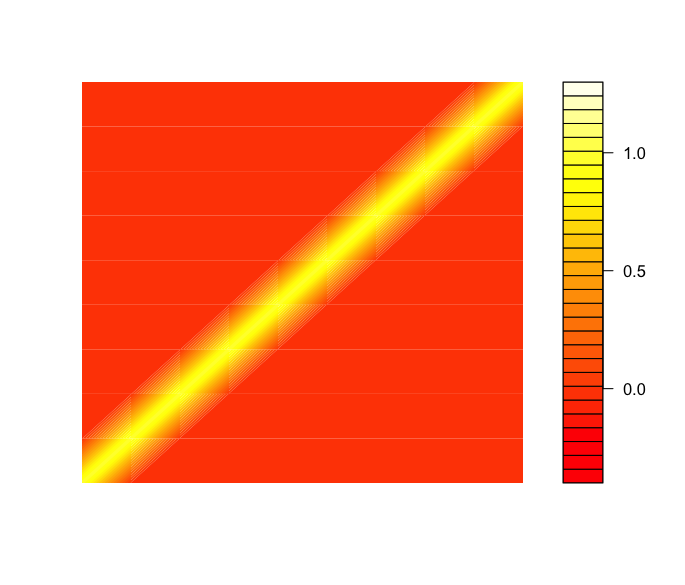
\includegraphics[width = \textwidth]{../img/chapter-4/true-covariance-1-heat-map}
%\label{fig:cattleA-regressogram-cubic-smooth}
%\caption{The sample regressogram for the cattle data from treatment group A, overlaid with a cubic polynomial smooth.}
\end{subfigure}
\hfill
  \begin{subfigure}[t]{0.19\textwidth}
\centering
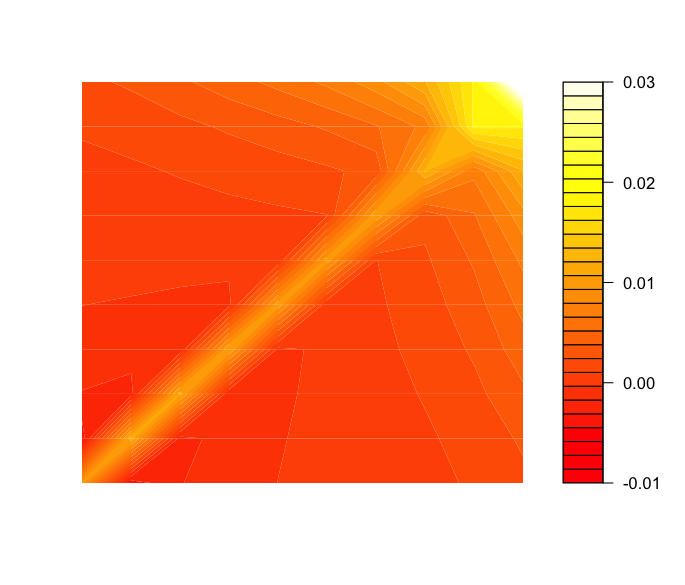
\includegraphics[width = \textwidth]{../img/chapter-4/true-covariance-2-heat-map}
%\label{fig:cattleA-regressogram-cubic-smooth}
%\caption{The sample regressogram for the cattle data from treatment group A, overlaid with a cubic polynomial smooth.}
\end{subfigure}
\hfill
  \begin{subfigure}[t]{.19\textwidth}
\centering
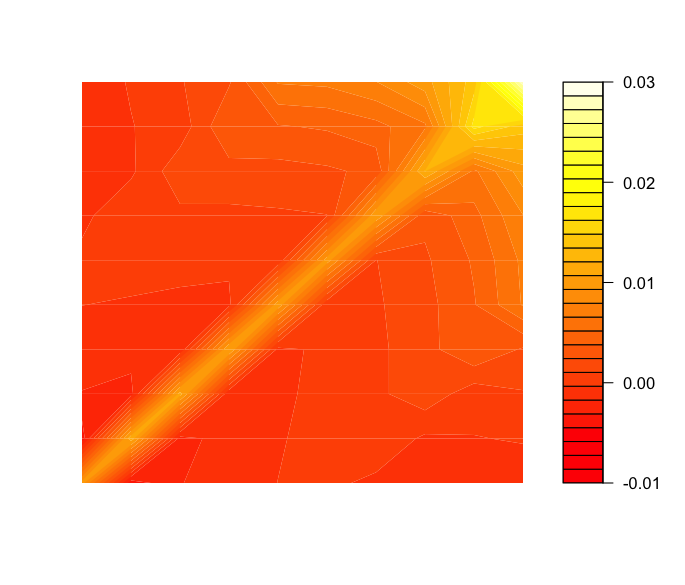
\includegraphics[width = \textwidth]{../img/chapter-4/true-covariance-3-heat-map}
%\label{fig:cattleA-regressogram-cubic-smooth}
%\caption{The sample regressogram for the cattle data from treatment group A, overlaid with a cubic polynomial smooth.}
\end{subfigure}
\hfill
  \begin{subfigure}[t]{0.19\textwidth}
\centering
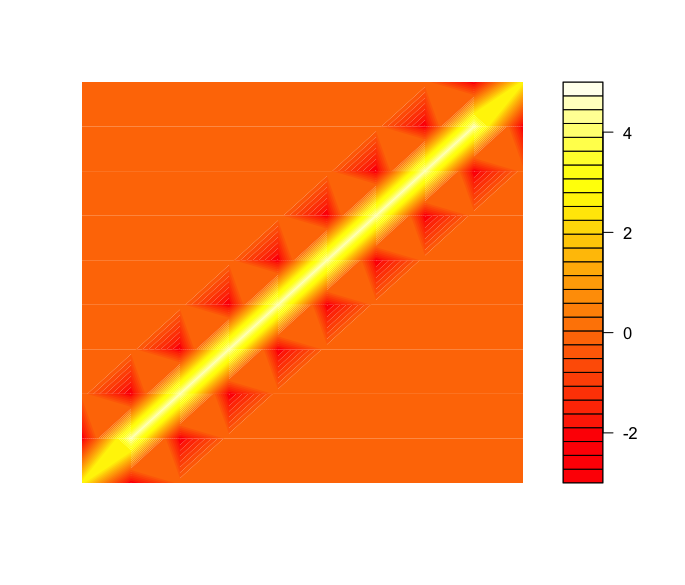
\includegraphics[width = \textwidth]{../img/chapter-4/true-covariance-4-heat-map}
%\label{fig:cattleA-regressogram-cubic-smooth}
%\caption{The sample regressogram for the cattle data from treatment group A, overlaid with a cubic polynomial smooth.}
\end{subfigure}
\hfill
  \begin{subfigure}[t]{0.19\textwidth}
\centering
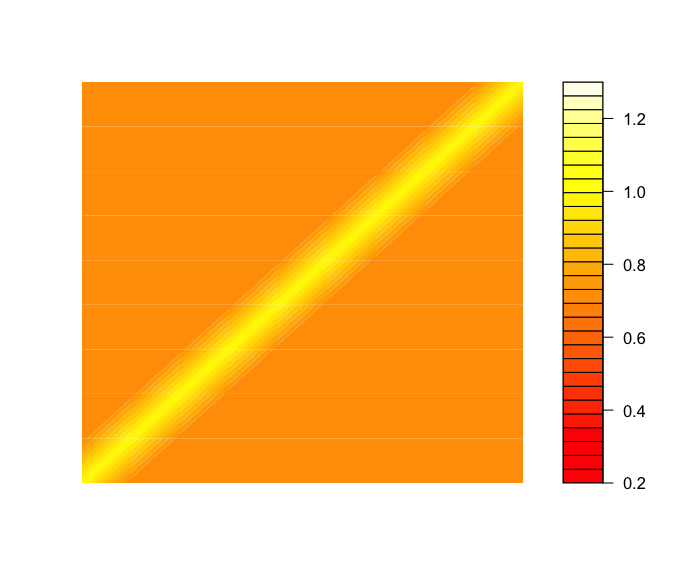
\includegraphics[width = \textwidth]{../img/chapter-4/true-covariance-5-heat-map}
%\label{fig:cattleA-regressogram-cubic-smooth}
%\caption{The sample regressogram for the cattle data from treatment group A, overlaid with a cubic polynomial smooth.}
\end{subfigure}
\end{figure}
